\section{Context}
The targeted environment is all work or educational environment. The analysis and design process will be based upon a university both the system should be easily implemented at any other work environment. 

\subsection{Problem Domain}
To fully understand the context we draw a rich picture which can be seen on figure \ref{fig:rich_picture}. 
The central aspects en the rich picture is that both the problem submitter and the problem solver can act on the problem, but will communicate through the system (the sharp with two documents). 
From the rich picture we see a few conflicts in the environment. 
The first is that problem exist but cannot be found. The second is that there could exist two similar problem. The central objects are the problems and solutions. 

\begin{figure}%
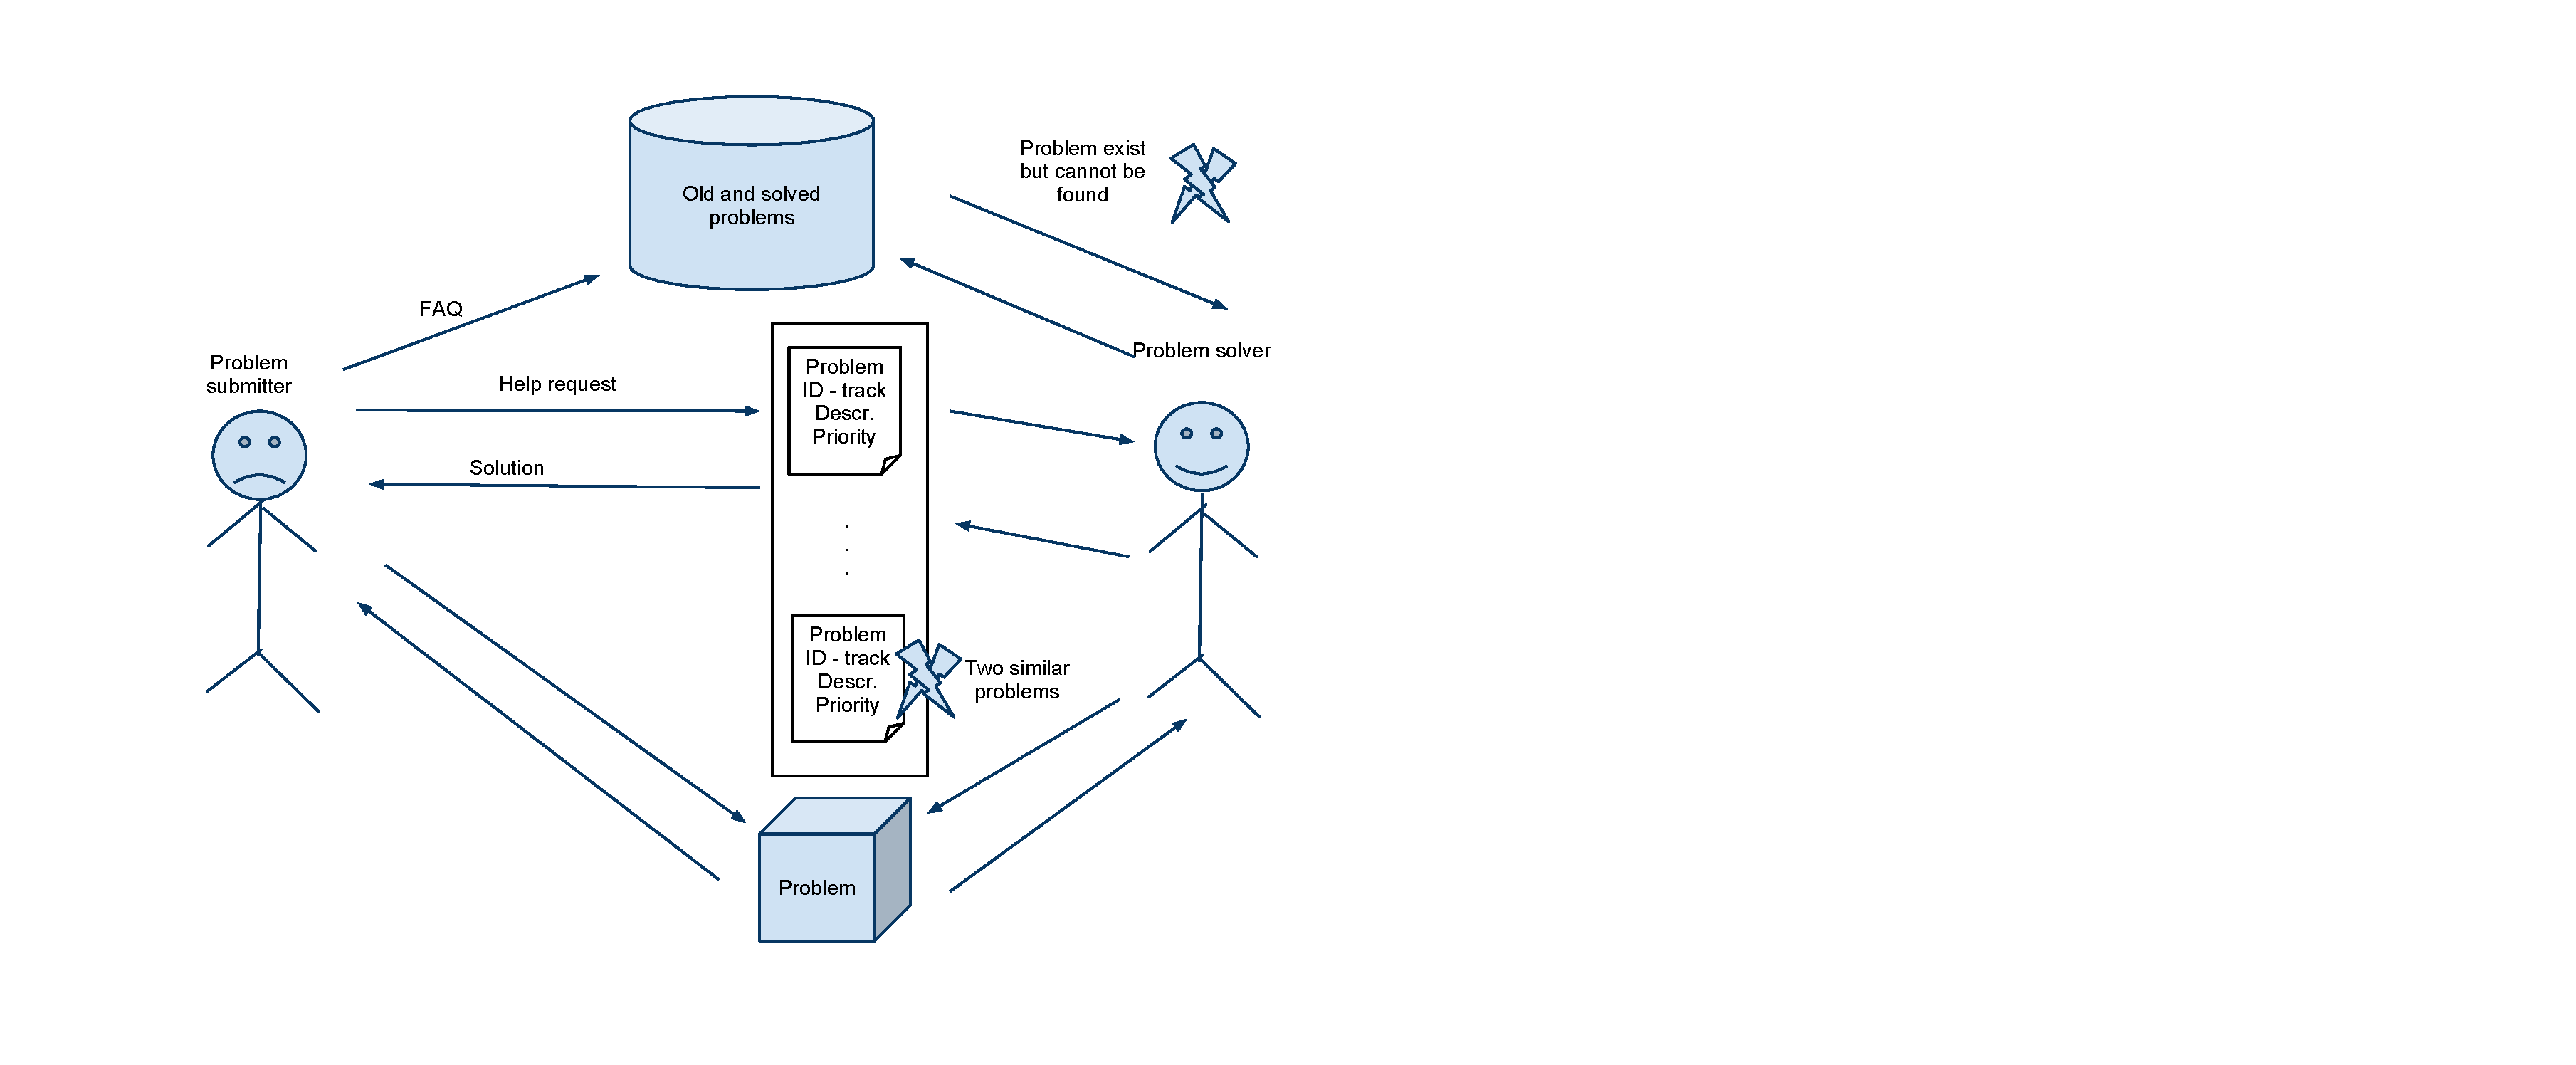
\includegraphics{input/background/rich_picture.pdf}%
\caption{Rich picture}%
\label{fig:rich_picture}%
\end{figure}

\subsection{Application Domain}
The people who will be acting on the system is the problem solver and submitter. Most likely the submitter will be a student in a university environment and the solver will be the technical staff. But the submitter could be a staff as well. Beside the two main actors there is an admin. Who can administrate the staff and clients. 